\documentclass[12pt]{article}


\usepackage[dvips,letterpaper,margin=0.75in,bottom=0.5in]{geometry}
\usepackage{cite}
\usepackage{slashed}
\usepackage{graphicx}
\usepackage{amsmath}

\begin{document}
\newcommand{\pt}           {\ensuremath{ p_{\rm T} }}
\newcommand{\Et}           {\ensuremath{ E_{\rm t}     }}

\let\divsymb=\div % rename builtin command \div to \divsymb
\newcommand{\gv}[1]{\ensuremath{\mbox{\boldmath$ #1 $}}} 
\newcommand{\grad}[1]{\gv{\nabla} #1} % for gradient
\renewcommand{\div}[1]{\gv{\nabla} \cdot #1} % for divergence


%\let\vaccent=\v % rename builtin command \v{} to \vaccent{}
%\renewcommand{\v}[1]{\ensuremath{\mathbf{#1}}} % for vectors
%\let\divsymb=\div % rename builtin command \div to \divsymb
%\newcommand{\uv}[1]{\ensuremath{\mathbf{\hat{#1}}}} % for unit vector
\newcommand{\abs}[1]{\left| #1 \right|} % for absolute value
\newcommand{\avg}[1]{\left< #1 \right>} % for average




\let\underdot=\d % rename builtin command \d{} to \underdot{}
\renewcommand{\d}[2]{\frac{d #1}{d #2}} % for derivatives
\newcommand{\dd}[2]{\frac{d^2 #1}{d #2^2}} % for double derivatives
\newcommand{\pd}[2]{\frac{\partial #1}{\partial #2}} % for partial derivatives
\newcommand{\pdd}[2]{\frac{\partial^2 #1}{\partial #2^2}} % for double partial derivatives
\newcommand{\pdc}[3]{\left( \frac{\partial #1}{\partial #2} \right)_{#3}} % for thermodynamic partial derivatives

\newcommand{\planewave}{e^{\textstyle i\vec{k} \cdot \vec{x}}}
\newcommand{\radialwave}{\frac{1}{r} \, e^{\textstyle ikr}} 

\title{Waves in One Dimension}
\author{Michael Mulhearn}

\maketitle

\section{Introduction}

If we throw a rock in water, we observe ripples.  If we pluck a taught
string, we hear and see the string vibrate.  When we talk, we produce
sound waves which travel through the air before reaching the ears of
our companions. These are all examples of waves, and while they differ
in details they share the same fundamental behavior: waves are
disturbances which travel through a medium.

\section{The Wave Equation}

A simple mathematical model for a medium which transmits waves
is a series of particles with mass $m$ connected by ideal springs of
constant $k$ and length $h$.  Define the $x$ axis to be along the direction of the springs, as in Fig.~\ref{fig:masses}.

\begin{figure}[thb]
\begin{center}
{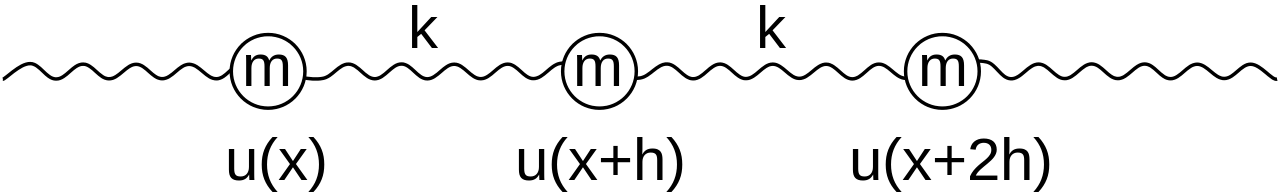
\includegraphics[width=0.55\textwidth]{figs/array_masses.png}}
\end{center}
\caption{\label{fig:masses} a model for a 1-D wave propagation.}
\end{figure}


We can model the wave as a disturbance of each mass from it's equilibrium position.  Imagine pulling on one of the small masses and then letting it go. There are two types of disturbances that we could make. If we pull a mass upward from its equilibrium position, the disturbance would be transverse to the medium, and we would create a transverse wave.  This would model waves on a taught string, and this calculation is already done in Unit E of Moore.  The other way we could disturb a mass is to push or pull the mass toward its neighbor, in the $+x$ or $-x$ direction, which would create a compressional wave.  Both of these are examples of 1-D waves, because  they propagate only along the $x$-axis, but in the compressional wave case, the geometric reasoning is much simpler.  We'll calculate the simpler compressional wave\footnote{This derivation and the figure are taken from http://en.wikipedia.org/wiki/Wave\_equation.}, but it turns out that you get the exact same wave equation, without too much more calculation, for transverse waves on a taught string.

We define $u(x,t)$ to be the amount that the mass with equilibrium position $x$ is offset from this position at time $t$.  This function $u(x,t)$ will be the equation describing our wave: it tells us how large the disturbance is at each point at each moment in time.

If we consider the particular mass with equilibrium position $x+h$, it has two forces acting upon it, from the two springs to its left and right, which connect it to the two masses which have equilibrium positions at $x$ and $x+2h$.  The force from the spring to the left is therefore:
\begin{displaymath}
F_{\rm left} = - k [ u(x+h,t) - u(x,t) ]
\end{displaymath}
which is easy to see if you recall that $u$ is the amount each mass is offset from its equilibrium (no force from the spring) position.  The force from the spring to the right is:
\begin{displaymath}
F_{\rm left} =  - k [ u(x+h,t) - u(x+2h,t) ]
\end{displaymath}
Next we note that the acceleration of the mass with equilibrium position $x+h$ is
\begin{displaymath}
a =  \pdd{u(x+h,t)}{t}
\end{displaymath}
So Newton's law 
\begin{displaymath}
{F_{\rm left} + F_{\rm right}} = m a
\end{displaymath}
becomes
\begin{displaymath}
m \pdd{u(x+h,t)}{t} = - k [ u(x+h,t) - u(x+2h,t)] - k [ u(x+h,t) - u(x,t)] 
\end{displaymath}
which simplifies to
\begin{displaymath}
\pdd{u(x+h,t)}{t} = \frac{k}{m} [ u(x+2h,t) - 2 u(x+h,t) + u(x,t)]
\end{displaymath}
That completes the microscopic picture of one mass.  Now we imagine that this system consists of $N$ such individual masses.  We are interested in the case where $N$ is a very large number, so that the space $h$ between each mass becomes very small, and we can think of $u$ as a continuous function.  

For a system of $N$ springs each with spring constant $k$, the total spring constant is $K = k/N$.  This is because if you pull on the large spring by an amount $\Delta X$, each individual spring would need to be displaced only by an amount $\Delta X / N$, so the force needed would be reduced by the factor $1/N$.  The total length and mass of the spring is given by $L = N h$ and $M = Nm$.  This leads to:
\begin{displaymath}
\frac{k}{m} = \frac{K L^2}{M} \cdot \frac{1}{h^2}
\end{displaymath}
which, when substituted in the previous equation, yields:
\begin{equation}\label{eqn:almost}
\pdd{u(x+h,t)}{t} = \frac{K L^2}{M} \cdot \frac{u(x+2h,t) - 2 u(x+h,t) + u(x,t)}{h^2}  
\end{equation}
To interpret this equation, we recall that the definition of a derivative is:
\begin{displaymath}
f'(x) = \lim_{h \to 0} \frac{f(x+h) - f(x)}{h} 
\end{displaymath}
From this definition, the second derivative must be
\begin{eqnarray*}
f''(x) & = & \lim_{h \to 0} \frac{f'(x+h) - f'(x)}{h} \\ 
& = & \lim_{h \to 0} \frac{\frac{f(x+2h) - f(x+h)}{h}-\frac{f(x+h) -f(x)}{h}}{h} \\
& = & \lim_{h \to 0} \frac{f(x+2h) - 2 f(x+h) + f(x)}{h^2} \\
\end{eqnarray*}
Comparing this to Equation \ref{eqn:almost} we conclude that in the limit of $h \to 0$, 
\begin{equation}
\pdd{u(x,t)}{t} = \frac{K L^2}{M} \cdot \pdd{u(x,t)}{x}
\end{equation}  
Dimensional analysis shows that the quantity $K L^2 / M$ has dimensions of velocity, so we define
\begin{equation}
v = \frac{K L^2}{M}
\end{equation}  
which leads to:
\begin{equation}\label{eqn:wave}
\frac{1}{v^2} \cdot \pdd{u(x,t)}{t} = \pdd{u(x,t)}{x} 
\end{equation}  
Equation~\ref{eqn:wave} is called a wave equation.  It is another example (like $F=ma$) of a differential equation.  The solutions to the wave equation are the waves $u(x,t)$ that could potentially propagate in this medium.  Although we derived it in a rather specific context, it comes up again and again in physics.  In the following section we'll show that the solutions to this equation are waves propagating in the plus or minus direction at a velocity given by the constant $v$.  

\section{A Solution to the Wave Equation}

A wave is, most generally, a disturbance which travels through a medium.  We can model the disturbance as a particular shape, parameterized by a function $f(x)$.  For the sake of this discussion, lets assume $f(x)$ is a particular shape with a maximum at $x=0$.  We can turn this shape into a wave by simply replacing $x$ with $x-v_x t$:

\begin{equation} \label{eqn:ansatz}
u(x,t) = f(x-v_x \, t)
\end{equation}
We can see that at a time $t$, the maximum of the shape ($f(0)$) will be located at the position $x$ such that $x-v_x t = 0$.  That is, at $x = v_x t$.  The peak of the wave is therefore traveling in the postive $x$ direction with velocity $v_x$, exactly like a wave.

Let's see if our intuition is correct, by seeing if Equation
\ref{eqn:ansatz} satisfies the wave Equation \ref{eqn:wave}.
\begin{eqnarray*}
\frac{1}{v^2} \cdot \pdd{u(x,t)}{t} & = & \pdd{u(x,t)}{x} \\
\frac{1}{v^2} \cdot \pdd{f(x-v_x \, t)}{t} & = & \pdd{f(x-v_x \, t)}{x} \\
\frac{v_x^2}{v^2} \cdot f''(x-v_x \, t) & = & f''(x-v_x \, t) \\ 
\end{eqnarray*}
This will be true provided $v_x^2 = v^2$, or $v_x = \pm v$.  We see therefore that any shape $f(x)$ is a solution to the wave equation if it propagates with the characteristic speed $v$ in either the plus or minus $x$ direction.  Specifically $f(x-v t)$ and $g(x+v t)$ are both solutions to the wave equation, for any functions $f(x)$ and $g(x)$.

\section{The Superposition Principle}

A crucial property of waves is that they pass through one another
undisturbed.  This property follows directly from the {\em linearity} of the wave equation.
If both $\alpha(x,t)$ and $\beta(x,t)$ are particular solutions to the wave equation, so that
\begin{equation} 
\frac{1}{v^2} \pdd{\alpha(x,t)}{t} = \pdd{\alpha(x,t)}{x}
\end{equation}  
and
\begin{equation}
\frac{1}{v^2} \pdd{\beta(x,t)}{t} = \pdd{\beta(x,t)}{x},
\end{equation}
it can be shown that $u(x,t) = A \alpha(x,t) + B \beta(x,t)$ also satisfies the
wave equation.  This calculation is left as an exercise below.

\section{The Superposition Principle and Boundary Conditions}

The superposition principle can be used to find solutions to otherwise challenging problems. Imagine a wave disturbance $u(x,t) = f(x-vt)$ traveling in the $+x$ direction and approaching the fixed end of the string at $x=0$.  We can model the end of the string as the condition that $u(0,t) = 0$. Because the string ends, the function $u(x,t)$ is undefined for $x>0$.  

This would be a very difficult problem to not for the superposition principle.  First we imagine that our string continues on past $x=0$ but arrange for a solution that always keeps $u(0,t) = 0$.   Once we have this solution, we ignore the function $u(x,t)$ above $x>0$.  To match the boundary conditions, we add to our right traveling wave $f(x-vt)$ a left traveling wave $g(x+vt)$.
\begin{displaymath}
u(x,t) = f(x-vt) + g(x+vt)
\end{displaymath}
We choose this left traveling wave to be the upside down reflection of the right traveling wave
\begin{displaymath}
g(x) = -f(-x) 
\end{displaymath}
or
\begin{displaymath}
u(x,t) = f(x-vt)  - f(-(x+vt))
\end{displaymath}
With this construction, we satisfy the boundary condition 
\begin{displaymath}
u(0,t) = f(0-vt)  - f(-(0+vt)) = f(-vt) - f(-vt) = 0
\end{displaymath}
If we look at how this appears for $x<0$ we see a wave approaching the end of the string, and being reflected backward with an inverted sign.  We simply ignore the solution to $u(x,t)$ above the end of the medium at $x>0$.

Another type of boundary condition is a free end.  In this case, the boundary condition is that the {\em slope} of the wave is zero at the open end.  In the case of a string terminated by a ring on a post, this is simply the observation that if the slope were non-zero, the ring would just slide up or down the post until the slope was zero (at an open end there is absolutely nothing pulling back in the transverse direction.)  

It is left as an exercise to show that the solution:
\begin{displaymath}
u(x,t) = f(x-vt)  + f(-(x+vt))
\end{displaymath}
satisfies the boundary condition that,
\begin{displaymath}
\left. \pd{u(x,t)}{x} \right|_{x=0} = 0.
\end{displaymath}
This shows that a wave encountering a free end of the medium is reflected backward without being inverted.

Another way we can encounter a boundary condition where the slope is zero is if we are {\em driving} the string from one end.  Imagine a flutist blowing on the end of flute, or someone jerking a rope up and down at one end.  In this case, the boundary condition is that the wave is maximal at the end, so the slope is zero.

\section{Sinusoidal Solutions to the Wave Equation}

\begin{figure}[thb]
\begin{center}
{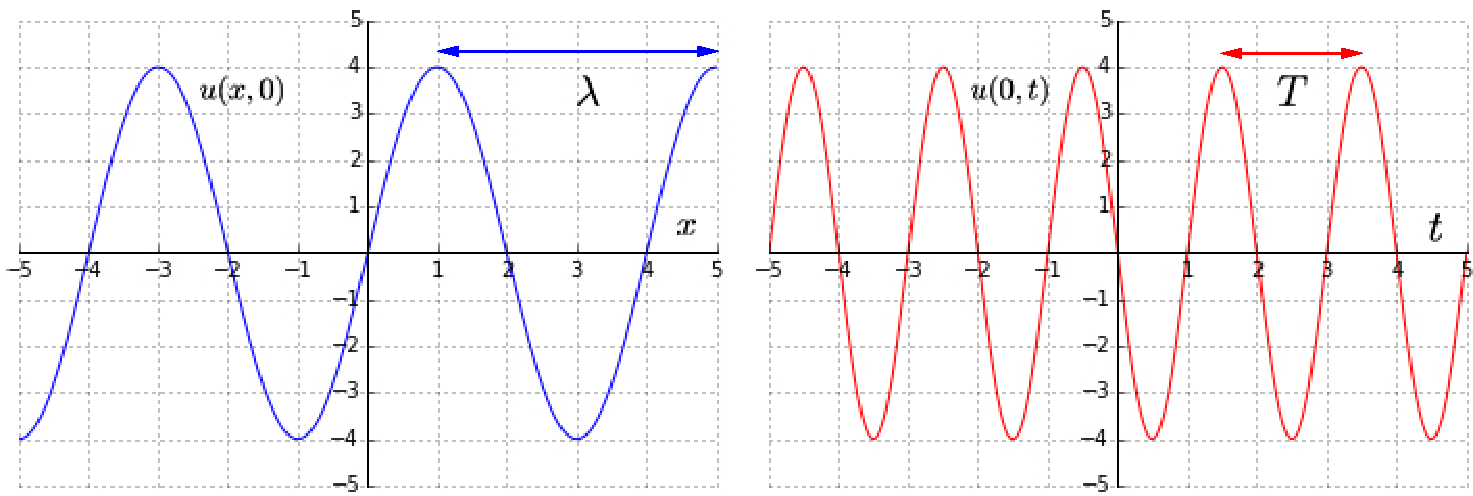
\includegraphics[width=0.95\textwidth]{figs/wave1d.pdf}}
\end{center}
\caption{\label{fig:sine wave} One way of visualizing the wave $u(x,t) = A \sin(k x-\omega t)$ with $A=4$, $k=\pi / 2$ and $\omega = \pi$.  The left plot shows the wave as a function of $x$ for $t=0$.  The right plot shows the value of the wave at the origin $x=0$ as a function of $t$.  This is a traveling wave with $\lambda = 4$ traveling to the right with a period of 2.}
\end{figure}

We have already shown that $f(x - v t)$ and $g(x + vt)$ are both solutions to the wave
equation for any functions $f(x)$ and $g(x)$.   In this section, we will consider a specific solution to the wave equation, which we write conventionally as:
\begin{equation}
u(x,t) = \sin(k x - \omega t).
\end{equation}
The wave is parameterized by $k$, which we call the {\em wave number}
and $\omega$, which we call the {\em angular frequency}.  
Writing the solution this way may seem strange to you, but you must get used to this convention, because you will see it again and again!   Note that this is indeed a solution to the wave equation, because we can write  
\begin{equation}
u(x,t) = \sin(k x - \omega t) = \sin \left(k \left(x - \frac{w}{k} \, t \right) \right) = f(x-vt)
\end{equation}
where the last step assumes that we have chosen $\omega$ and $k$ such that:
\begin{equation}
v = \frac{\omega}{k}.
\end{equation}

As shown if Fig.~\ref{fig:sine wave}, the parameters of a wave are:
\begin{itemize}
 \item The maximum height of the wave, which we call the amplitude, $A$.
 \item The distance between two successive peaks, which we call the wavelength $\lambda$.
 \item The time it takes the wave to complete one entire cycle, which we call the period $T$.
\end{itemize}
To see how these relate to the wave number, $k$, and the angular frequency $\omega$, we note that the sine function has a period of $2 \pi$ radians.  So when x advances by the wavelength $\lambda$, we must have $k \lambda$ advance by $2 \pi$ to complete exactly one cycle.  Hence:
\begin{equation}
k = \frac{2 \pi}{ \lambda}.
\end{equation}
Likewise, when $t$ advances by one period $T$, we must $\omega T$ advance by $2 \pi$, so that
\begin{equation}
\omega = \frac{2 \pi}{ T}.
\end{equation}
The frequency $f$, which is measured in Hertz (${\rm H} = {\rm s}^-1$) is defined as:
\begin{equation}
f= \frac{1}{ T},
\end{equation}
so we can also write the angular frequency as
\begin{equation}
\omega = 2 \pi f.
\end{equation}

Finally, note that the velocity of the wave is 
\begin{equation}
v = \frac{\omega}{k} = \frac{\lambda}{T} ,
\end{equation}
which makes sense, as the wave takes one period to travel a distance of one wavelength.


\section{Separable Solutions to the Wave Equation}

Suppose that the $x$ and $t$ dependence of a wave are separable, by which we mean we can write:
\begin{equation}
u(x,t) = f(x) g(t).
\end{equation}
In order to satisfy the wave equation (Equation~\ref{eqn:wave}), we must therefore have 
\begin{eqnarray*}
\frac{1}{v^2} \cdot \pdd{f(x)g(t)}{t} & = & \pdd{f(x)g(t)}{x}  \\
\frac{f(x)}{v^2} \cdot \dd{g(t)}{t} & = & g(t) \cdot \dd{f(x)}{x}  \\
\frac{f(x)}{v^2} \cdot g''(t) & = & g(t) \cdot f''(x)  \\
\frac{1}{v^2} \cdot \frac{g''(t)}{g(t)} & = & \frac{f''(x)}{f(x)}  \\
\end{eqnarray*}
Look closely at the last step.  The left-hand side is a function of $t$ only, while the right-hand side is a function of $x$ only.  The only way this equality can be satisfied, therefore, is if both of these expressions are equal to the same constant value $C$.  This constant has the dimensions of one over distance squared, or a wave-number squared, so we might as well set $C = \pm k^2$.  We don't know the sign of the constant.  It turns out that the useful solutions come from choosing $C = -k^2$ (You'll look at the case $C = +k^2$ in the exercises.) 

We now have two separate differential equations to solve (this is progress??!!).  The first one is:
\begin{eqnarray*}
\frac{f''(x)}{f(x)} & = & -k^2\\
f''(x) & = & -k^2 \cdot f(x) \\
\end{eqnarray*}
and the second is: 
\begin{eqnarray*}
\frac{g''(t)}{g(t)} & = & -v^2 k^2 = -\omega^2 \\
g''(t)& = & -\omega^2 g(t)\\
\end{eqnarray*}
Our familiar sine function is a solution to this equation
\begin{eqnarray}
f(x) & =  & a \sin (kx + \alpha) \\
g(t) & = & b \sin (\omega t + \beta) \\
\end{eqnarray}
where $a$,$b$,$\alpha$, and $\beta$ are constants.  A combined solution to the wave equation is just the product of these two functions:
\begin{equation}\label{eqn:separable}
u(x,t) = A \sin (kx + \alpha) \sin (\omega t + \beta)
\end{equation}
where $A$,$\alpha$, and $\beta$ are the constants.  Note that $\alpha$
and $\beta$ are phases of the sine waves, so for instance choosing
$\alpha=\pi/2$ or $\beta=\pi/2$ has the same effect as switching the
sine for a cosine.



\section{Standing-Wave Solutions to the Wave Equation}

\begin{figure}[thb]
\begin{center}
{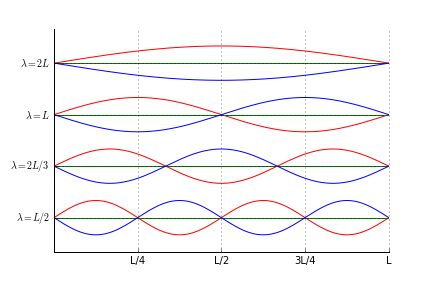
\includegraphics[width=0.50\textwidth]{figs/harmonics.png}}
\end{center}
\caption{\label{fig:harmonics} First four standing waves with fixed-ends a length $L$ apart.  The waves oscillate (red, green, blue, green, red) with a period given by $T = \lambda/v$.}
\end{figure}

\noindent
Consider a right traveling wave
\begin{equation}
u_R(x,t) = \sin(k x - \omega t)
\end{equation}
which is traveling in medium from $x = -\infty$ that ends suddenly at $x=0$ such that $u(0,t) = 0$.  We saw previously that satisfying this fixed-end boundary condition will require a reflected (left traveling) inverted wave:
\begin{equation}
u_L(x,t) = -\sin(-k x - \omega t) = \sin(k x + \omega t) 
\end{equation}
The complete solution to the wave equation that satisfies this boundary condition is therefore
\begin{eqnarray*}
u(x,t) & = & u_L(x,t) + u_R(x,t)  \\
& = &  \sin(k x - \omega t) + \sin(k x + \omega t)\\
& = &  \sin(k x) \cos( \omega t) - \cos(k x) \sin( \omega t) + \sin(k x) \cos( \omega t) + \cos(k x) \sin( \omega t) \\
& = & 2 \sin(k x ) \cos(\omega t).
\end{eqnarray*}
This is the same solution as Equation~\ref{eqn:separable} with $A=2$, $\alpha=0$, and $\beta=\pi/2$. 

The solutions we obtained by assuming the wave was separable are the standing wave solutions.  Physically, these waves do not move, they have fixed shape $\sin(kx+\alpha)$ with an amplitude that is changing with time.  Because standing waves have nodes (and peaks) located at fixed points, they are ideal solutions to the wave equation for a medium with end points.  One merely chooses the particular standing waves that are appropriate for the particular boundary conditions of interest.

For instance, consider a taught string held fixed at $x=0$ and $x=L$.  The first four solutions to the wave equation (ordered with decreasing wavelength) are shown in Fig.~\ref{fig:harmonics}.  The largest wavelength solution is for $\lambda = 2 L$, which has only two nodes, at the positions $x=0$ and $x=L$.  The next solution, with wavelength $L$ adds a node at $x=L/2$.  The complete set of possible wavelengths are:
\begin{equation}
\lambda_n = 2 L / n
\end{equation}
where $n=1,2,3,...$

\section{Fourier Series}

\begin{figure}[thb]
\begin{center}
{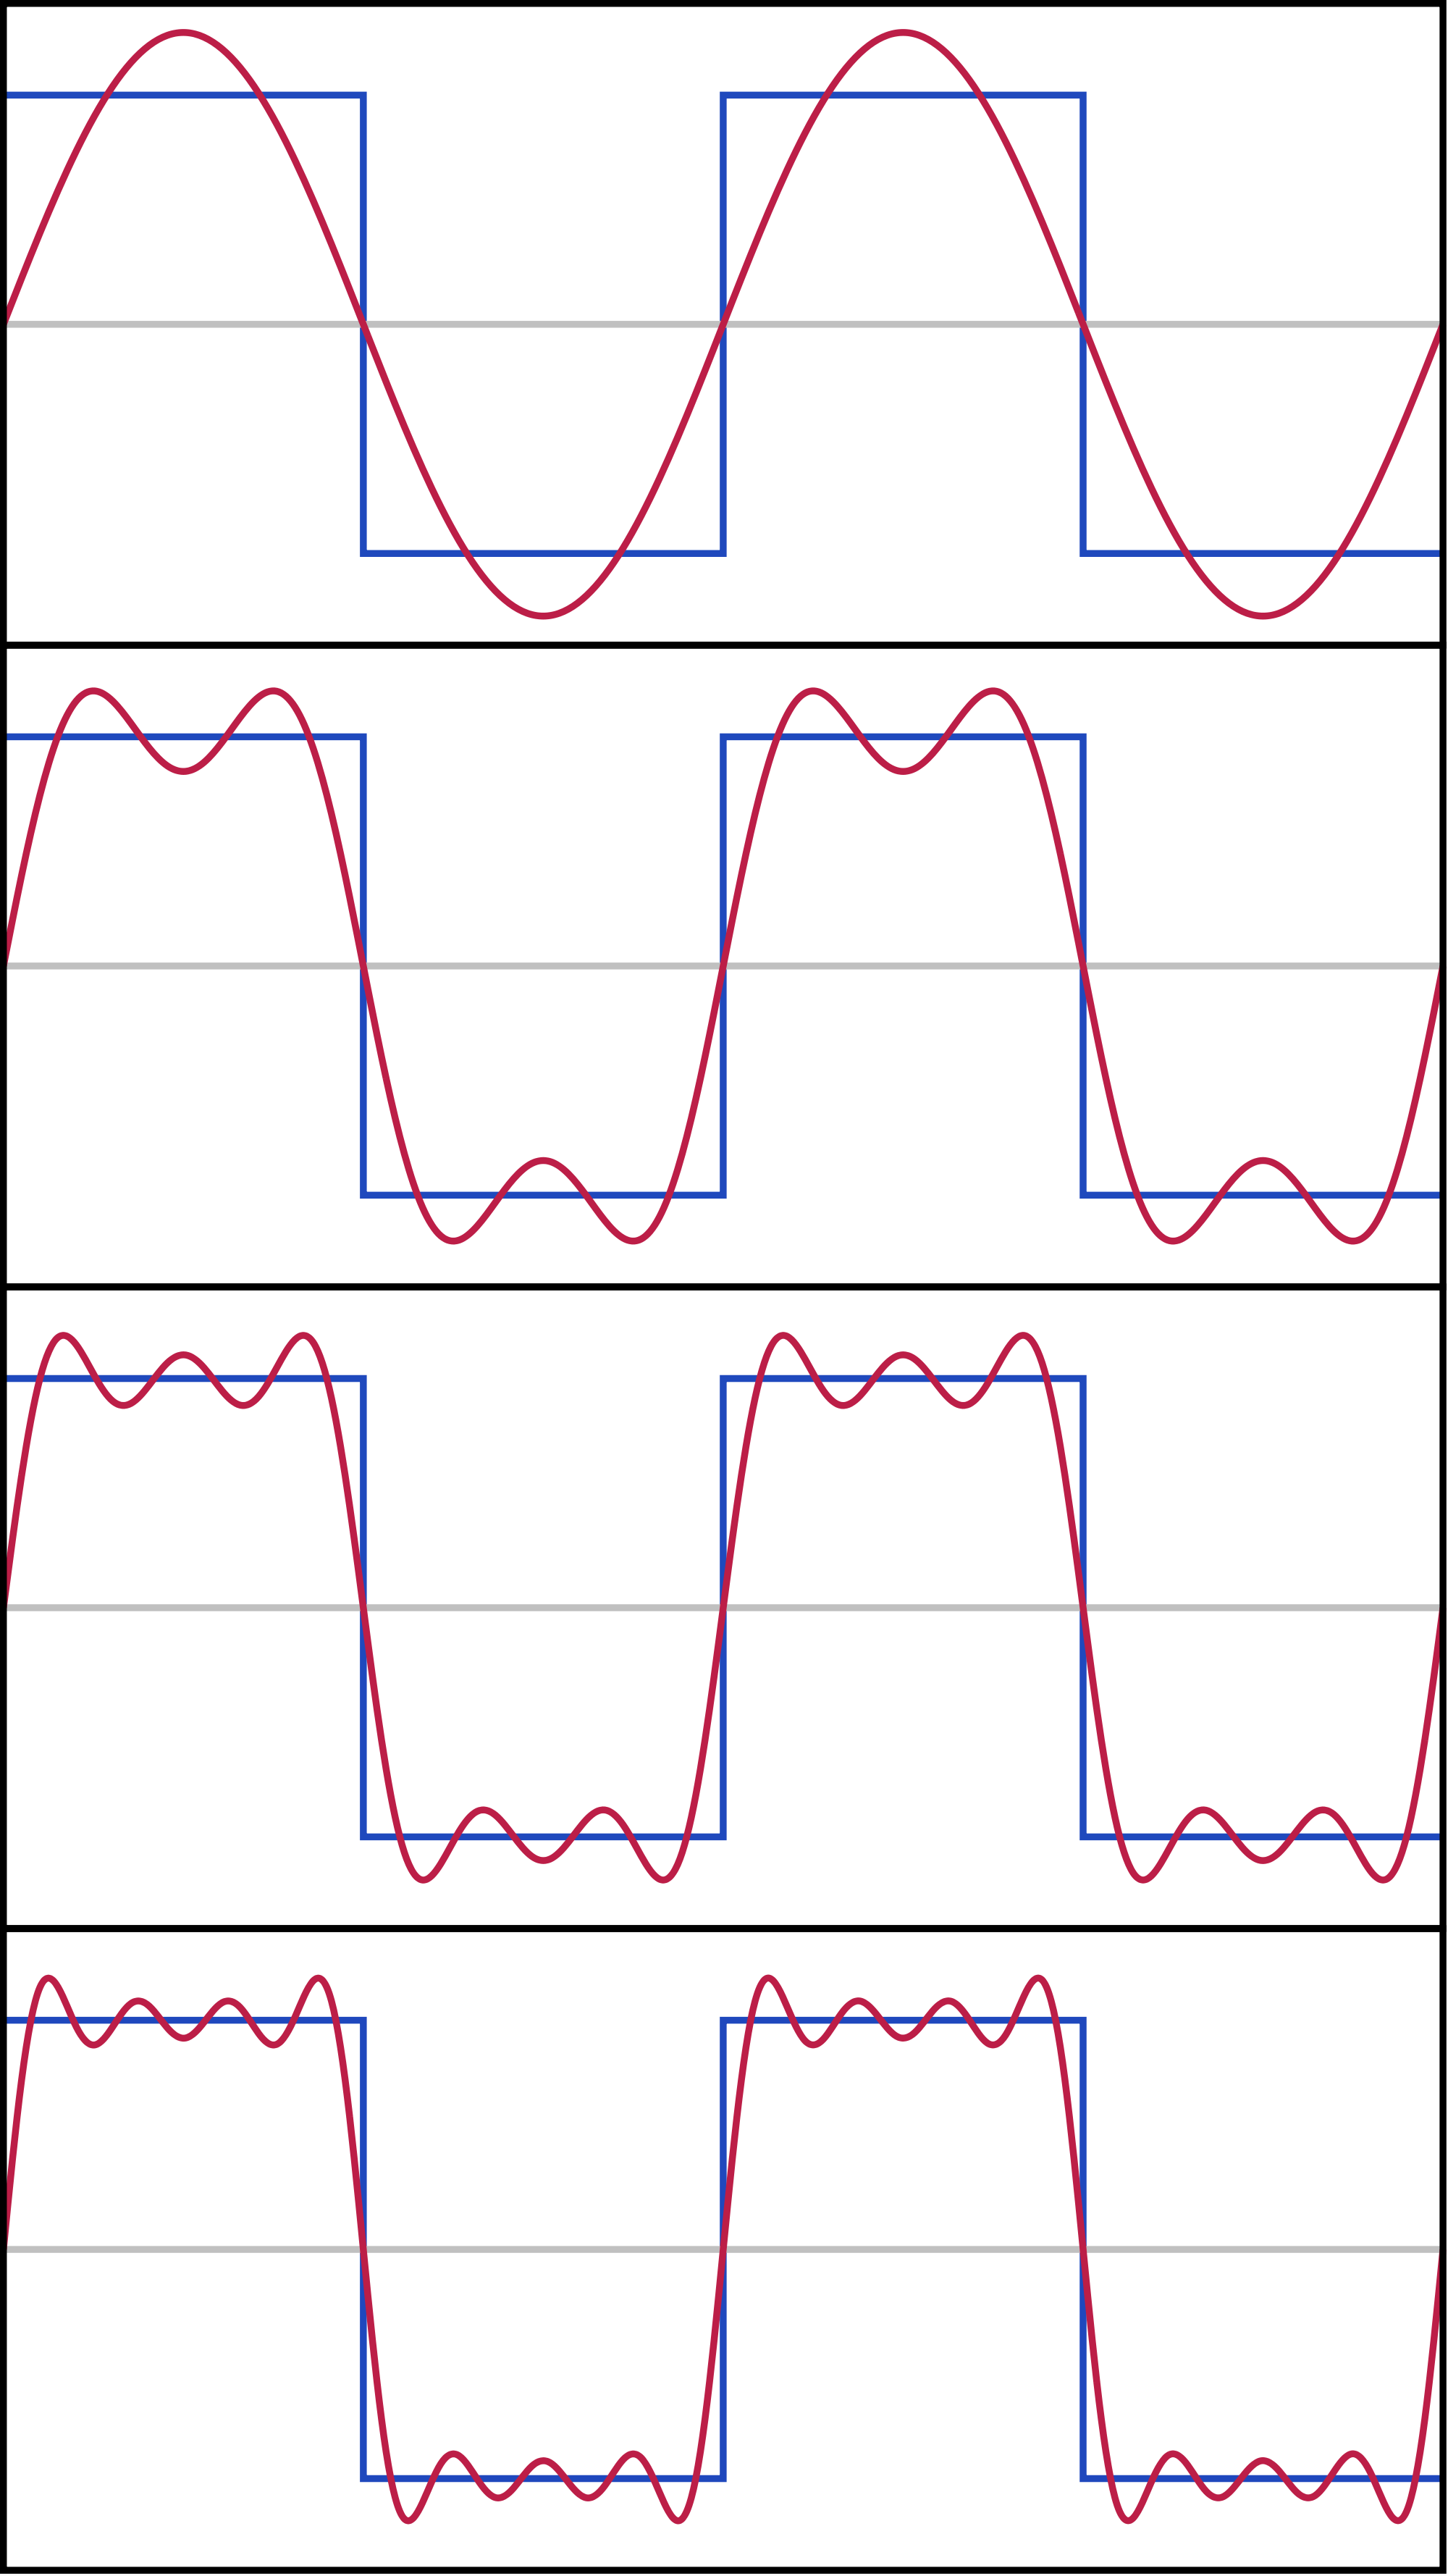
\includegraphics[width=0.30\textwidth]{figs/fourier.png}}
\end{center}
\caption{\label{fig:fourier} An example showing the approximation of a periodic square function from the first four terms in the Fourier series.}
\end{figure}

The sinusoidal functions (sines and cosines) are just one possible solution to the wave equation.  But it turns out they are extremely important because they have a very special property.   Any periodic function can be approximated {\em to any desired precision} as a series of sine and cosine functions.   If $f(x)$ has the property that $f(x+L) = f(x)$, then
\begin{equation}
f(x) = \sum_{n=0}^\infty a_n \cos \left(\frac{n \pi x }{L} \right) + \sum_{n=1}^\infty b_n \sin \left(\frac{n \pi x}{L} \right)
\end{equation}
This is called the Fourier Series.  Mathematically, we say that the sines and cosines are {\em complete}, because you can build any function you need out of them by simply adding them together in the right combination.  An example is shown in Fig.~\ref{fig:fourier}.

There is a general prescription for determining the the coefficients $a_n$ and $b_n$, but we shall leave that for later.   The reason for introducing this idea now is merely to explain, in a qualitative way, that by providing the sine and cosine solutions to the wave equations, we have in fact provided the complete set of solutions to the wave equation.

\section{Energy Density of a Wave}

Recall that our model for a wave consisted of a series of masses and
springs.  The equilibrium distance between each spring is $h$ (and we
will eventually take the limit $h \to 0$.)

The energy associated with a mass nominally at position $x$ is purely kinetic energy,
\begin{displaymath}
K = \frac{1}{2} m \left( \pd{u(x,t)}{t} \right)^2,
\end{displaymath}
while the energy associated with a spring connecting the mass nominally at position $x$ with the mass nominal at position $x+h$ is purely potential energy:
\begin{displaymath}
U = \frac{1}{2} k [u(x+h,t) - u(x,t)]^2.
\end{displaymath}
These two contribution are the total energy associated with a length
$h$ of the system\footnote{It might trouble you that the masses are
 not necessarily exactly a distance $h$ apart when not in the
 equilibrium positions, but keep in mind that our wave $u(x,t)$ is still only
 defined at the discrete points $0,h,2h,3h,...$, so we are implicitly
 assuming the oscillations are small enough that we can treat each mass as if
 it was at effectively at its equilibrium positon}, so we can calculate the energy density as
\begin{displaymath}
\mu = \frac{K + U}{h} = \frac{1}{2} \frac{m}{h} \left( \pd{u(x,t)}{t} \right)^2 + \frac{1}{2} k h \left( \frac{u(x+h)-u(x)}{h}\right)^2 
\end{displaymath}
Now using $M=Nm$, $L=Nh$, $K=k/N$, and $v = K L^2 / M$ this can be written:
\begin{displaymath}
\mu = \frac{1}{2} \frac{M}{L} \left( \left(\pd{u(x,t)}{t}\right)^2 + v^2 \left( \frac{u(x+h)-u(x)}{h} \right)^2\right) 
\end{displaymath}
And taking the limit $h \to 0$ we get
\begin{equation}\label{eqn:edensity}
\mu = \frac{1}{2} \frac{M}{L} \left( \left(\pd{u(x,t)}{t}\right)^2 + v^2 \left( \pd{u(x,t)}{x} \right)^2\right) 
\end{equation}

\section{Exercises}

\noindent
{\em Problem 1:} Show that the functions $u(x,t) = a x$ and $u(x,t) =
b t$, with $a$ and $b$ both constants, are also solutions to the wave equation.  Provide a physical
interpretation of each of these solutions. \\

\vskip 0.5cm

\noindent
{\em Problem 2:} Show explicitly that if $\alpha(x,t)$ and $\beta(x,t)$ each satisfy the wave equation, then the function $u(x,t) = A \alpha(x,t) + B \beta(x,t)$ is also a solution. \\

\vskip 0.5cm

\noindent
{\em Problem 3:} Show that the solution to the wave equation:
\begin{displaymath}
u(x,t) = f(x-vt)  + f(-(x+vt))
\end{displaymath}
satisfies the boundary condition that,
\begin{displaymath}
\pd{u(x,t)}{x} |_{x=0} = 0
\end{displaymath}. \\

\noindent
{\em Problem 4:}   Verify that $\cos(kx - \omega t)$ satisfies the wave equation as long as $k = \pm \omega / v$. \\

\vskip 0.5cm

\noindent
{\em Problem 5:}   Is $u(x,t) = \cos(kx + \omega t)$ a wave moving in the $+x$ direction or in the $-x$ direction? Assume both $k$ and $\omega$ are positive numbers. \\

\vskip 0.5cm


\noindent
{\em Problem 6:} Write down the expression for a standing sinusoidal
wave on a taught string with fixed ends at $x=-L/2$ and $x=L/2$.  The
wave has amplitude $A$, has six nodes, and reaches a maximum at $t=0$.
(Hint: use the general solution Equation~\ref{eqn:separable}, find
appropriate values of $k$, $\omega$, $\alpha$, and $\beta$.)  

\vskip 0.5cm

\noindent
{\em Problem 7:}   A {\em quarter-wave antenna} uses standing waves to produce radio waves in the atmosphere.  One end of the antenna is driven by an electrical circuit, so it is an antinode.  The other end of the antenna comes to an abrupt end, so it is a node.  Sketch the $x$ dependance of the first three harmonics (as in Fig.~\ref{fig:harmonics}) of a quarter wave antenna.  Does the term quarter-wave antenna make sense?

\vskip 0.5cm

\noindent
{\em Problem 8:}
In the section on Separable Solutions to the wave equation, we found solutions to the differential equations for the case $C=-k^2$.  What are the solutions to the wave equation if this constant is positive $C=k^2$?

\vskip 0.5cm

\noindent
{\em Problem 9:}   It turns out you have been using Fourier's Theorem since you were in grade school!  The function $f(x) = \sin(kx + \theta)$, where $\theta$ is just some constant, is a periodic function in $x$.  Fourier's Theorem tells us that we should be able to express $f(x)$ as a sum of $\sin(nkx)$ and $\cos(nkx)$.  In fact, this is a very simple case where there are only two terms in the sum, so that
\begin{displaymath}
\sin(kx+\theta) = a \sin(kx) + b \cos(kx)
\end{displaymath}
Use a grade school trigonometric identity to find the constants $a$ and $b$ in terms of $\theta$. \\

\vskip 1cm

\noindent
{\em Problem 10:}  Consider the right-traveling sinusoidal wave $u(x,t) = A \sin(kx - \omega t)$.  Compute the average energy density by calculating the total energy stored in one wave-length and dividing by the wave length:
\begin{displaymath}
\mu_{\rm avg} = \frac{1}{\lambda} \cdot \int_0^\lambda \mu \; dx
\end{displaymath}
(Hint: Use Equation~\ref{eqn:edensity}.  You can perform the integration at $t=0$.) 
\end{document}




